\documentclass[11pt,spanish]{article} % Idioma
\usepackage{babel}
\usepackage[T1]{fontenc}
\usepackage{textcomp}
\usepackage[utf8]{inputenc} % Puede depender del instrucción, sistema o editor
\usepackage{wrapfig} % Imagenes
% \graphicspath{ {./imagenes/} }

\usepackage[left=2.75cm,top=2.5cm,right=2cm,bottom=2.5cm]{geometry} % Márgenes
%\usepackage{pstricks} % Gráficas, movilidad, árboles y otros

\usepackage{amssymb, amsmath} % Símbolos matemáticos
\usepackage{amsthm} % Teoremas, lemas, pruebas...
\usepackage{cancel} % Cancelar expresiones
\usepackage{multirow} % Tablas
\usepackage{graphicx} % Inserción de imágenes
\usepackage{xcolor} % Colores
\usepackage{color}
\definecolor{gray97}{gray}{.97}
\definecolor{gray75}{gray}{.75}
\definecolor{gray45}{gray}{.45}

\usepackage[hidelinks]{hyperref}  % Enlaces
\usepackage{multirow} % Tablas

\usepackage{listings} % Escribir código en diferentes lenguajes de programación
\lstset{ frame=Ltb,
framerule=0pt,
aboveskip=0.5cm,
framextopmargin=3pt,
framexbottommargin=3pt,
framexleftmargin=0.4cm,
framesep=0pt,
rulesep=.4pt,
backgroundcolor=\color{gray97},
rulesepcolor=\color{black},
%
stringstyle=\ttfamily,
showstringspaces = false,
basicstyle=\small\ttfamily,
commentstyle=\color{gray45},
keywordstyle=\bfseries,
%
numbers=left,
numbersep=15pt,
numberstyle=\tiny,
numberfirstline = false,
breaklines=true,
}

\title{Memoria de algor\'itmica}
\author{Rubén Morales Pérez
		\and Francisco Javier Morales Piqueras
		\and Bruno Santindrian Manzanedo
		\and Ignacio de Loyola Barragan Lozano
		\and Francisco Leopoldo Gallego Salido}
\date{\today}


% % % % % % % % % % % % % % % % % % % % % % % % % % % % % % % % %
%					 Inicio del documento
% % % % % % % % % % % % % % % % % % % % % % % % % % % % % % % % %
\begin{document}
\maketitle
\tableofcontents % Generando el indice
\newpage
\setlength\parindent{0pt} % Quitamos la sangría

%%%%%%%%%%%%%%%%%%%%%%%%%%%%%%%%%%%%%%%%%%%%%%%%%%%%%%%%%%%%%%%%%%%%%%%%%%%%%%%%%%


\section{Explicaci\'on del m\'etodo utilizado}
Para la obtenci\'on de los datos deseados hemos realizado un script de bash que genera las tablas de datos y las gráficas con su correspondiente ajuste.
\begin{lstlisting}[language=bash]
#!/bin/bash

if [ $# -ne 1 ]
then
    echo "Uso: $0 <nombre>"
    exit 1
fi

# HEAPSORT
g++ -std=c++11 ../src/heapsort.cpp
nelementos=200
echo "" > datos.dat
while [ $nelementos -lt 10000 ]; do
    ./a.out $nelementos >> datos.dat
    let nelementos=nelementos+100
done

gnuplot ./gnuplot/heapsort.gp # Salida: "fichero.jpeg"

mkdir ../Graficas/Heapsort 2> /dev/null
mkdir ../Graficas/Heapsort/Datos 2> /dev/null
mv fichero.jpeg ../Graficas/Heapsort/heapsortO0_$1.jpeg
mv datos.dat ../Graficas/Heapsort/Datos/heapsortO0_$1.dat
echo "Heapsort completado"


# MERGESORT
g++ -std=c++11 ../src/mergesort.cpp
nelementos=200
echo "" > datos.dat
while [ $nelementos -lt 10000 ]; do
    ./a.out $nelementos >> datos.dat
    let nelementos=nelementos+100
done

gnuplot ./gnuplot/mergesort.gp # Salida: "fichero.jpeg"

mkdir ../Graficas/Mergesort 2> /dev/null
mkdir ../Graficas/Mergesort/Datos 2> /dev/null
mv fichero.jpeg ../Graficas/Mergesort/mergesortO0_$1.jpeg
mv datos.dat ../Graficas/Mergesort/Datos/mergesortO0_$1.dat
echo "Mergesort completado"


# INSERCION
g++ -std=c++11 ../src/insercion.cpp
nelementos=200
echo "" > datos.dat
while [ $nelementos -lt 10000 ]; do
    ./a.out $nelementos >> datos.dat
    let nelementos=nelementos+100
done

gnuplot ./gnuplot/insercion.gp # Salida: "fichero.jpeg"

mkdir ../Graficas/Insercion 2> /dev/null
mkdir ../Graficas/Insercion/Datos 2> /dev/null
mv fichero.jpeg ../Graficas/Insercion/insercionO0_$1.jpeg
mv datos.dat ../Graficas/Insercion/Datos/insercionO0_$1.dat
echo "Insercion completado"


# SELECCION
g++ -std=c++11 ../src/seleccion.cpp
nelementos=200
echo "" > datos.dat
while [ $nelementos -lt 10000 ]; do
    ./a.out $nelementos >> datos.dat
    let nelementos=nelementos+100
done

gnuplot ./gnuplot/insercion.gp # Salida: "fichero.jpeg"

mkdir ../Graficas/Seleccion 2> /dev/null
mkdir ../Graficas/Seleccion/Datos 2> /dev/null
mv fichero.jpeg ../Graficas/Seleccion/seleccionO0_$1.jpeg
mv datos.dat ../Graficas/Seleccion/Datos/seleccionO0_$1.dat
echo "Seleccion completado"


# QUICKSORT
g++ -std=c++11 ../src/quicksort.cpp
nelementos=200
echo "" > datos.dat
while [ $nelementos -lt 10000 ]; do
    ./a.out $nelementos >> datos.dat
    let nelementos=nelementos+100
done

gnuplot ./gnuplot/quicksort.gp # Salida: "fichero.jpeg"

mkdir ../Graficas/Quicksort 2> /dev/null
mkdir ../Graficas/Quicksort/Datos 2> /dev/null
mv fichero.jpeg ../Graficas/Quicksort/quicksortO0_$1.jpeg
mv datos.dat ../Graficas/Quicksort/Datos/quicksortO0_$1.dat
echo "Quicksort completado"


# BURBUJA
g++ -std=c++11 ../src/burbuja.cpp
nelementos=200
echo "" > datos.dat
while [ $nelementos -lt 10000 ]; do
    ./a.out $nelementos >> datos.dat
    let nelementos=nelementos+100
done

gnuplot ./gnuplot/burbuja.gp # Salida: "fichero.jpeg"

mkdir ../Graficas/Burbuja 2> /dev/null
mkdir ../Graficas/Burbuja/Datos 2> /dev/null
mv fichero.jpeg ../Graficas/Burbuja/burbujaO0_$1.jpeg
mv datos.dat ../Graficas/Burbuja/Datos/burbujaO0_$1.dat
echo "Burbuja completado"


# FIBONACCI
g++ -std=c++11 ../src/fibonacci.cpp
nelementos=1
echo "" > datos.dat
while [ $nelementos -lt 50 ]; do
    ./a.out $nelementos >> datos.dat
    let nelementos=nelementos+2
done

gnuplot ./gnuplot/fibonacci.gp # Salida: "fichero.jpeg"

mkdir ../Graficas/Fibonacci 2> /dev/null
mkdir ../Graficas/Fibonacci/Datos 2> /dev/null
mv fichero.jpeg ../Graficas/Fibonacci/fibonacciO0_$1.jpeg
mv datos.dat ../Graficas/Fibonacci/Datos/fibonacciO0_$1.dat
echo "Fibonacci completado"


# HANOI
g++ -std=c++11 ../src/hanoi.cpp
nelementos=3
echo "" > datos.dat
while [ $nelementos -lt 30 ]; do
    ./a.out $nelementos >> datos.dat
    let nelementos=nelementos+1
done

gnuplot ./gnuplot/hanoi.gp # Salida: "fichero.jpeg"

mkdir ../Graficas/Hanoi 2> /dev/null
mkdir ../Graficas/Hanoi/Datos 2> /dev/null
mv fichero.jpeg ../Graficas/Hanoi/hanoiO0_$1.jpeg
mv datos.dat ../Graficas/Hanoi/Datos/hanoiO0_$1.dat
echo "Hanoi completado"


# FLOYD
g++ -std=c++11 ../src/floyd.cpp
nelementos=200
echo "" > datos.dat
while [ $nelementos -lt 1000 ]; do
    ./a.out $nelementos >> datos.dat
    let nelementos=nelementos+10
done

gnuplot ./gnuplot/floyd.gp # Salida: "fichero.jpeg"

mkdir ../Graficas/Floyd 2> /dev/null
mkdir ../Graficas/Floyd/Datos 2> /dev/null
mv fichero.jpeg ../Graficas/Floyd/floydO0_$1.jpeg
mv datos.dat ../Graficas/Floyd/Datos/floydO0_$1.dat
echo "Floyd completado"

rm a.out
rm fit.log
\end{lstlisting}

Para la obtención de las gráficas de forma directa utilizamos script de gnuplot que tienen la forma siguiente, en este caso adjuntamos "burbuja.gp".

\begin{lstlisting}[language=gnuplot]
set terminal jpeg
set output "fichero.jpeg"

set title "Eficiencia burbuja"
set xlabel "Tamano del vector"
set ylabel "Tiempo (s)"
set fit quiet
f(x) = a*x*x+b*x+c
fit f(x) "datos.dat" via a, b, c
plot "datos.dat", f(x)
\end{lstlisting}

Los diferentes ajustes se han conseguido así:

\begin{lstlisting}[language=gnuplot]
f(x) = a*x*x*x+b*x*x+c*x+d
g(x) = a*x*x+b*x+c
h(x) = a*x*(log(x)/log(2))
i(x) = a*(((1+sqrt(5))/2)**x)
\end{lstlisting}


\newpage
%%%%%%%%%%%%%%%%%%%%%%%%%%%%%%%%%%%%%%%%%%%%%%%%%%%%%%%%%%%%%%%%%%%%%%%%%%%%%%%%%%

\section{C\'alculo de la eficiencia emp\'irica}
%\hspace*{1cm}\textbf{Ejercicio 1.}

\subsection{Tabla con los algor\'itmos cuadr\'aticos}
\subsection{Tabla con los algor\'itmos c\'ubicos}
\subsection{Tabla con los algor\'itmos nlog(n)}
\subsection{Tabla con el algor\'itmo de Fibonacci}
\begin{table}[htb]
\centering
\begin{tabular}{|l|l|}
\hline
\multicolumn{2}{|c|}{Fibonaccii} \\ \hline
1 & 2 \\
\hline \hline
t11 & t12 \\ \hline
t21 & t22 \\ \hline
\end{tabular}
\caption{Tabla de tiempos}
\label{tabla:fib}
\end{table}

\subsection{Tabla con el algor\'itmo de Hanoi}
\subsection{Tabla con los algoritmos de ordenaci\'on}

\newpage
%%%%%%%%%%%%%%%%%%%%%%%%%%%%%%%%%%%%%%%%%%%%%%%%%%%%%%%%%%%%%%%%%%%%%%%%%%%%%%%%%%

\section{Gr\'aficas}

\subsection{Ordenaci\'ion}
En este apartado compararemos 6 algoritmos diferentes de ordenación dentro de un vector.
Cada algoritmo lleva su ajuste correspondiente.

\subsubsection{Burbuja}
$f(x) = a\cdot x^2 + b\cdot x + c \implies$
$\left\{ \begin{array}{c}
a               = 4.31433\cdot 10^{-9}      +/- 2.378\cdot 10^{-10}    (5.511\%) \\
b               = 3.94506\cdot 10^{-6}      +/- 2.476\cdot 10^{-6}    (62.75\%) \\
c               = -0.00311235      +/- 0.005425     (174.3\%)
\end{array}\right.$
\begin{center}
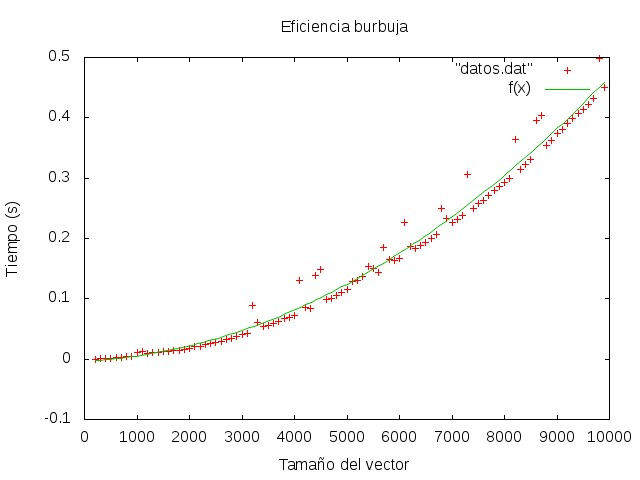
\includegraphics[scale=0.55]{../Graficas/Burbuja/burbujaO0_ruben.jpeg}
\end{center}

\subsubsection{Inserci\'on} %%%%%%%%%%%%%%%%%%%%%%%%%%%%%%%%%%%%%%%%55
$f(x) = a\cdot x^2 + b\cdot x + c \implies$
$\left\{ \begin{array}{c}
a               = 2.36229\cdot 10^{-9}      +/- 2.503\cdot 10^{-10}    (10.6\%) \\
b               = -2.27723\cdot 10^{-6}     +/- 2.606\cdot 10^{-6}    (114.5\%) \\
c               = 0.00096037       +/- 0.005712     (594.8\%)
\end{array}\right.$

\begin{center}
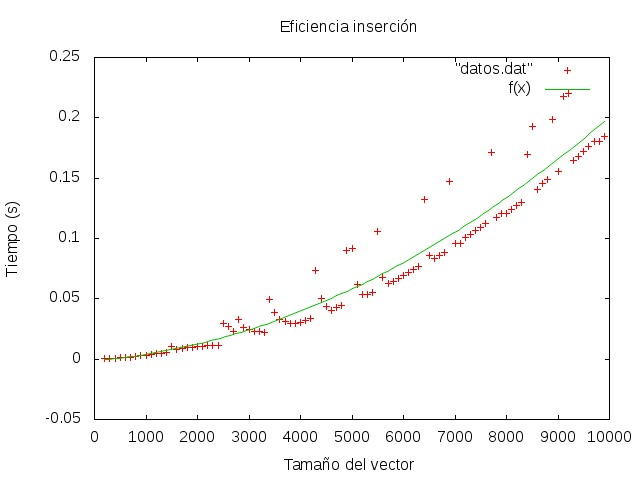
\includegraphics[scale=0.55]{../Graficas/Insercion/insercionO0_ruben.jpeg}
\end{center}

\newpage
\subsubsection{Selecci\'on}
$f(x) = a\cdot x^2 + b\cdot x + c \implies$
$ a               = 2.36327\cdot 10^{-9}      +/- 3.232\cdot 10^{-11}    (1.368\%) $
\begin{center}
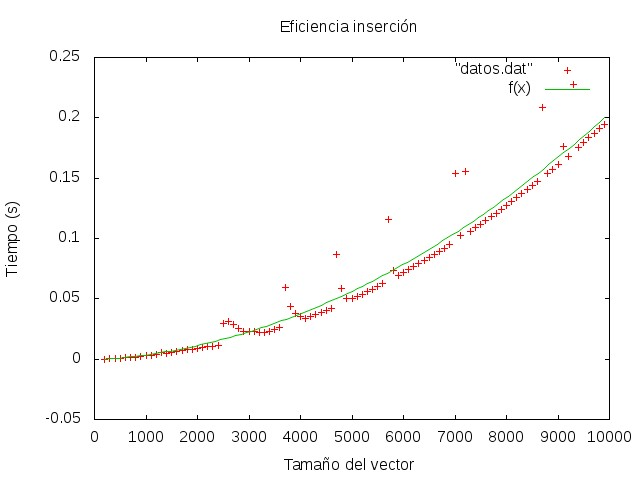
\includegraphics[scale=0.55]{../Graficas/Seleccion/seleccionO0_ruben.jpeg}
\end{center}

{\ }

\subsubsection{Mergesort}
$ f(x) = a\cdot x\cdot log_2(x) \implies$
$ a               = 3.5231\cdot 10^{-8}       +/- 1.191\cdot 10^{-9}    (3.382\%) $
\begin{center}
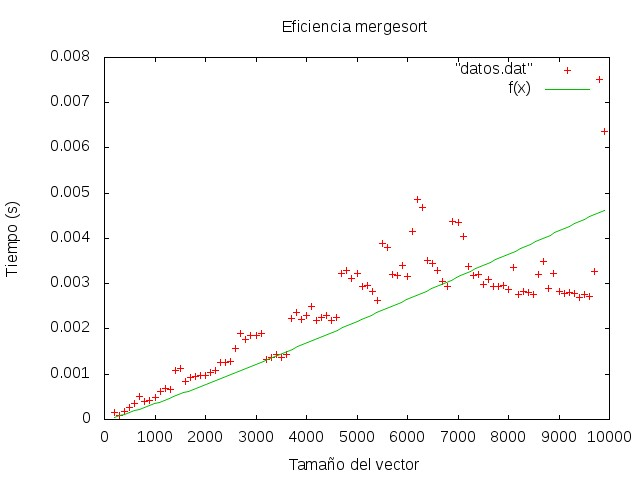
\includegraphics[scale=0.55]{../Graficas/Mergesort/mergesortO0_ruben.jpeg}
\end{center}
\newpage

\subsubsection{Quicksort}
$ f(x) = a\cdot x\cdot log_2(x) \implies$
$ a               = 2.3704\cdot 10^{-8}       +/- 5.497\cdot 10^{-10}    (2.319\%) $
\begin{center}
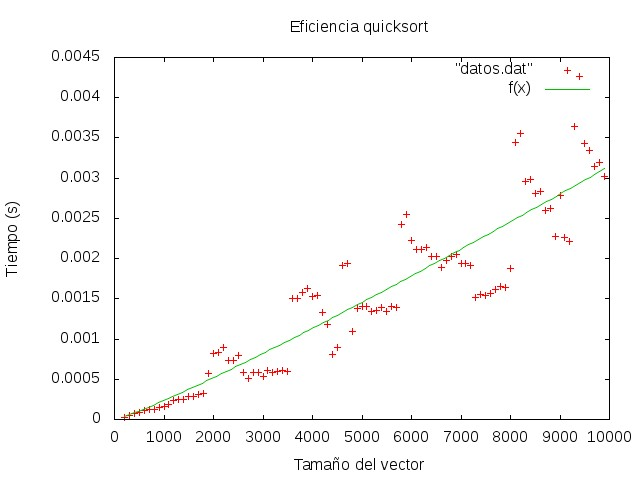
\includegraphics[scale=0.55]{../Graficas/Quicksort/quicksortO0_ruben.jpeg}
\end{center}

\subsubsection{Heapsort}
$ f(x) = a\cdot x\cdot log_2(x) \implies$
$a               = 2.49016\cdot 10^{-8}      +/- 7.983\cdot 10^{-10}    (3.206\%)$
\begin{center}
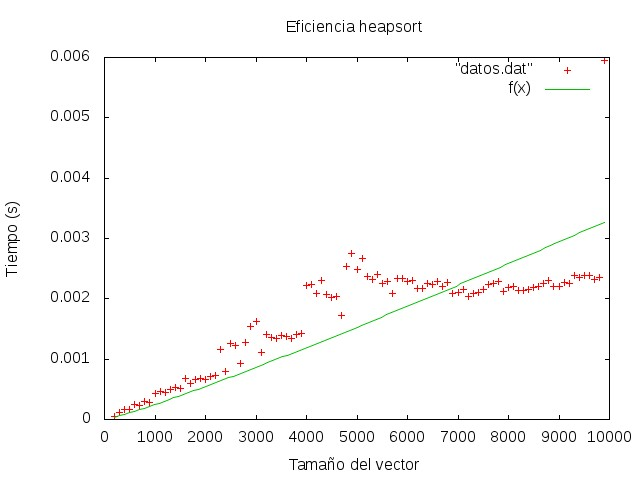
\includegraphics[scale=0.55]{../Graficas/Heapsort/heapsortO0_ruben.jpeg}
\end{center}

\subsubsection{Comparativa algoritmos de ordenaci\'ion}

En este apartado comprobamos empíricamente las diferencias de eficiencia entre diferentes algoritmos de ordenación de un vector. Se observa una diferencia notable entre los algoritmos $O(nlog_2(n))$ y los $O(n^2)$, casi no se aprecian los primeros.

También nos percatamos de la diferencia dentro de los mismos algoritmos con eficiencia $O(n^2)$, debido a la constante multiplicativa que los acompaña, inserción y selección son parecidos y burbuja tarda bastante más que los anteriores.

\begin{center}
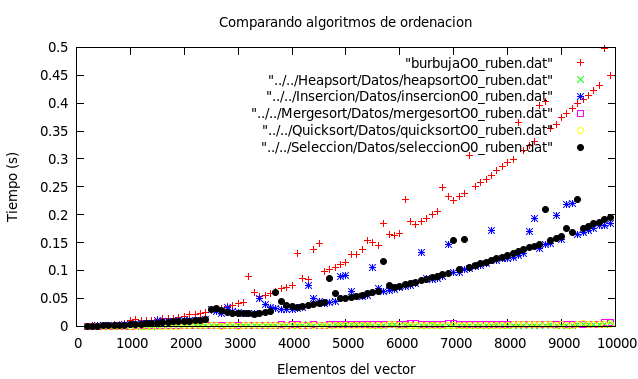
\includegraphics[scale=0.55]{../Graficas/todos.png}
\end{center}

\subsection{Fibonacci}
$ f(x) = a\cdot ((1+\sqrt(5))/2)^x \implies$
$a               = 5.59738\cdot 10^{-9}      +/- 2.093\cdot 10^{-12}    (0.0374\%)$

\begin{center}
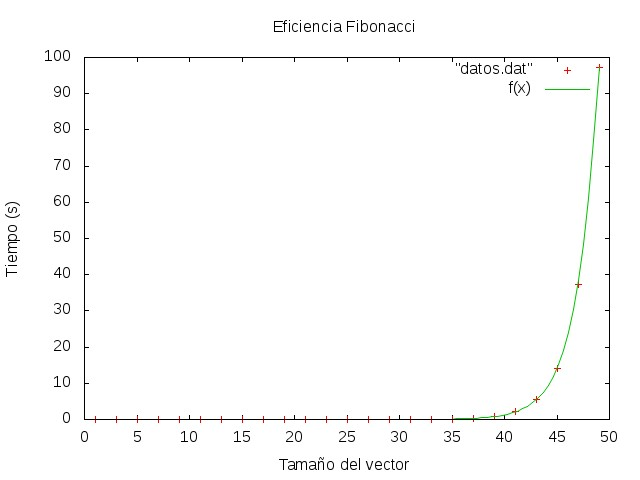
\includegraphics[scale=0.55]{../Graficas/Fibonacci/fibonacciO0_ruben.jpeg}
\end{center}
\newpage
\subsection{Hanoi}
$f(x) = a\cdot(2^x) \implies$
$a               = 1.12636\cdot 10^{-8}      +/- 1.391\cdot 10^{-11}    (0.1235\%)$
\begin{center}
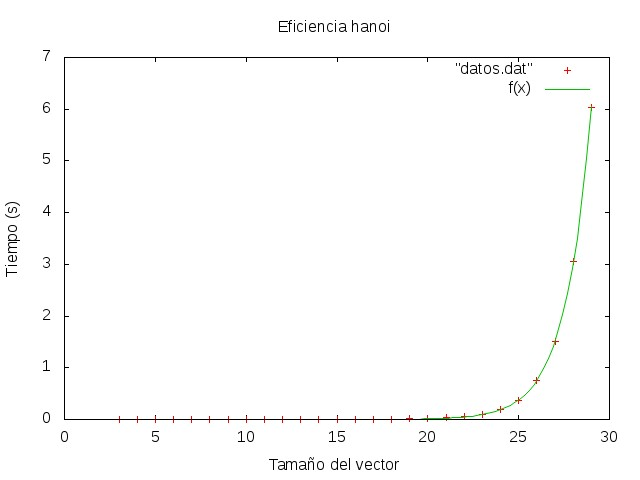
\includegraphics[scale=0.55]{../Graficas/Hanoi/hanoiO0_ruben.jpeg}
\end{center}


\subsection{Floyd}
$f(x) = a\cdot x^3 + b\cdot x^2 + c\cdot x + d \implies$
$\left\{ \begin{array}{c}
a               = 1.11725\cdot 10^{-8}      +/- 3.725\cdot 10^{-10}    (3.334\%) \\
b               = -2.27723\cdot 10^{-6}     +/- 6.692\cdot 10^{-7}    (29.39\%) \\
c               = 0.00096037       +/- 0.0003713    (38.66\%) \\
d               = -0.115743        +/- 0.06234      (53.86\%)
\end{array}\right.$

\begin{center}
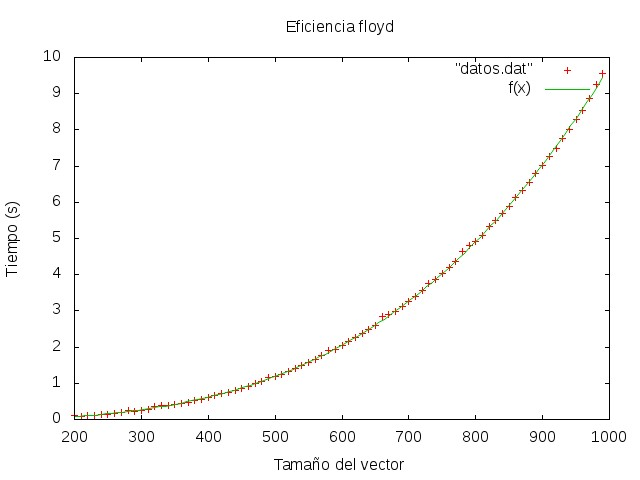
\includegraphics[scale=0.55]{../Graficas/Floyd/floydO0_ruben.jpeg}
\end{center}
\newpage

\subsection{Optimizaci\'on de algunos algoritmos}
Como podemos comprobar, por mucho que optimicemos el algoritmo de burbuja no llega a igualarse al mejor algoritmo de ordenación (en término medio), quicksort. La optimización más agresiva sin riesgo de pérdida de información es -O2 y llega a ser 10 veces más lento que quicksort sin optimización (con 10.000 elementos).

Esto es una prueba gráfica de que hay que tener en cuenta la eficiencia de los algoritmos, ya que la mejora hardware no es suficiente en caso de que tengamos restricciones de tiempo.

\begin{center}
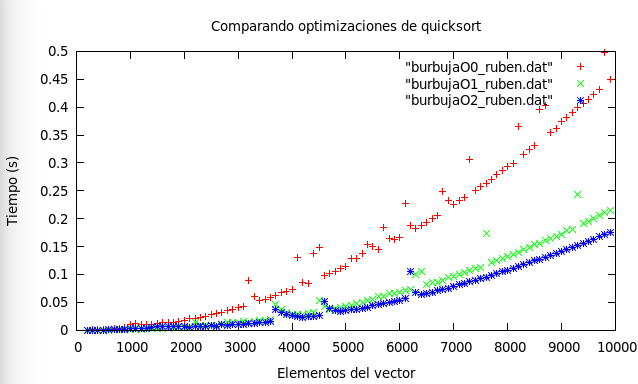
\includegraphics[scale=0.55]{../Graficas/Burbuja/burbuja_optimizacion.png}
\end{center}

Una observación curiosa es que el algoritmo Quicksort realmente es un algoritmo con eficiencia en el caso peor de $O(n^2)$, ya que si le pasamos un vector que está ordenado es cuadrático. Por otro lado Heapsort es un $O(nlog_2n)$ puro, pero en término medio es peor que Quicksort, ya que los datos que se suelen pasar a estos algoritmos no están ordenados.

\begin{center}
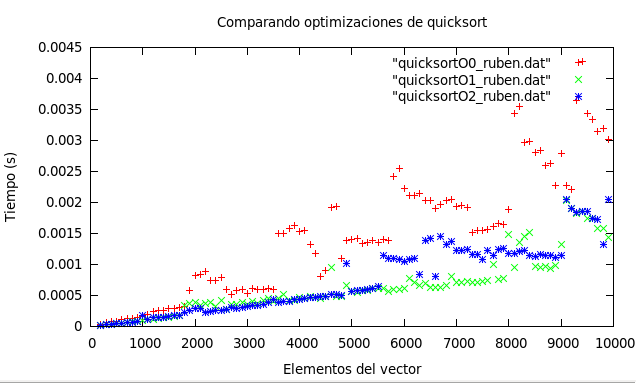
\includegraphics[scale=0.55]{../Graficas/Quicksort/quicksort_optimizacion.png}
\end{center}

{\ }

Después de comparar dichos algoritmos de ordenación optimizaremos el algoritmo floyd, tipo de algoritmo con programación dinámica para encontrar el camino mínimo en grafos ponderados.

\begin{center}
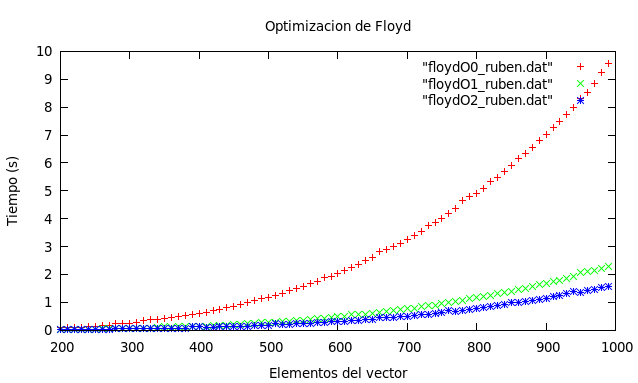
\includegraphics[scale=0.55]{../Graficas/Floyd/floyd_optimizacion.png}
\end{center}


\section{Ordenador usado para la ejecuci\'on}
HP Pavilion g series (Pavilion g6)

Sistema operativo: ubuntu 14.04 LTS

Memoria: 3.8 GiB (4Gb)

Procesador: Inter Core i3-2330M CPU @ 2.20GHz x 4

Gráficos: Intel Sandybridge Mobile

Tipo de SO: 64 bits

Disco: 487.9 GB

\newpage
%%%%%%%%%%%%%%%%%%%%%%%%%%%%%%%%%%%%%%%%%%%%%%%%%%%%%%%%%%%%%%%%%%%%%%%%%%%%%%%%%%

% % % % % % % % % % % % % % % % % % % % % % % % % % % % % % % % %
%					 Bibliografía
% % % % % % % % % % % % % % % % % % % % % % % % % % % % % % % % %
% input{bibliografia}

\end{document}
